\chapter{Evaluation and Results}
\label{chapter:evaluation_and_results}


The objective for this chapter is to validate the proposed solution. Firstly, in section \ref{results:scenario}, a deployment scenario overview will be given, highlighting the devices and tools used for that purpose. Following, in section \ref{results:results}, the obtained results for different tests will be analysed. With the requirements, addressed in chapter 3, taken into consideration, the performance of the automation engine, implemented in gateways, will be evaluated, and also, to judge the capacity of the system to react to abnormal functioning scenarios, the reaction time to this occurrences will be measured.

\newpage

\section{Deployment Scenario}
\label{results:scenario}



The final deployment scenario, used to test and validate the system and illustrated in Figure \ref{fig:performance}, is composed by the Building Manager platform, the WSO2 \ac{cep} Engine, the Gateway Manager and two Gateways, all communicating through the MQTT Broker. 

The Building Manager is the component responsible for supporting the user-friendly platform to create rules and distribute devices through the building planer. This platform was hosted in a Linux virtual machine equipped with a single-core processor and 1 gigabyte of memory.

The WSO2 \ac{cep} engine, which is one of the core components of the whole system, as it is the primary processor of events, based on the logic specified in the rules. This component, required a more powerful machine than the Building Manager component , being hosted in a Linux virtual machine with a quad-core processor and 4 gigabytes of memory.

\begin{figure}[H]
	\centering
	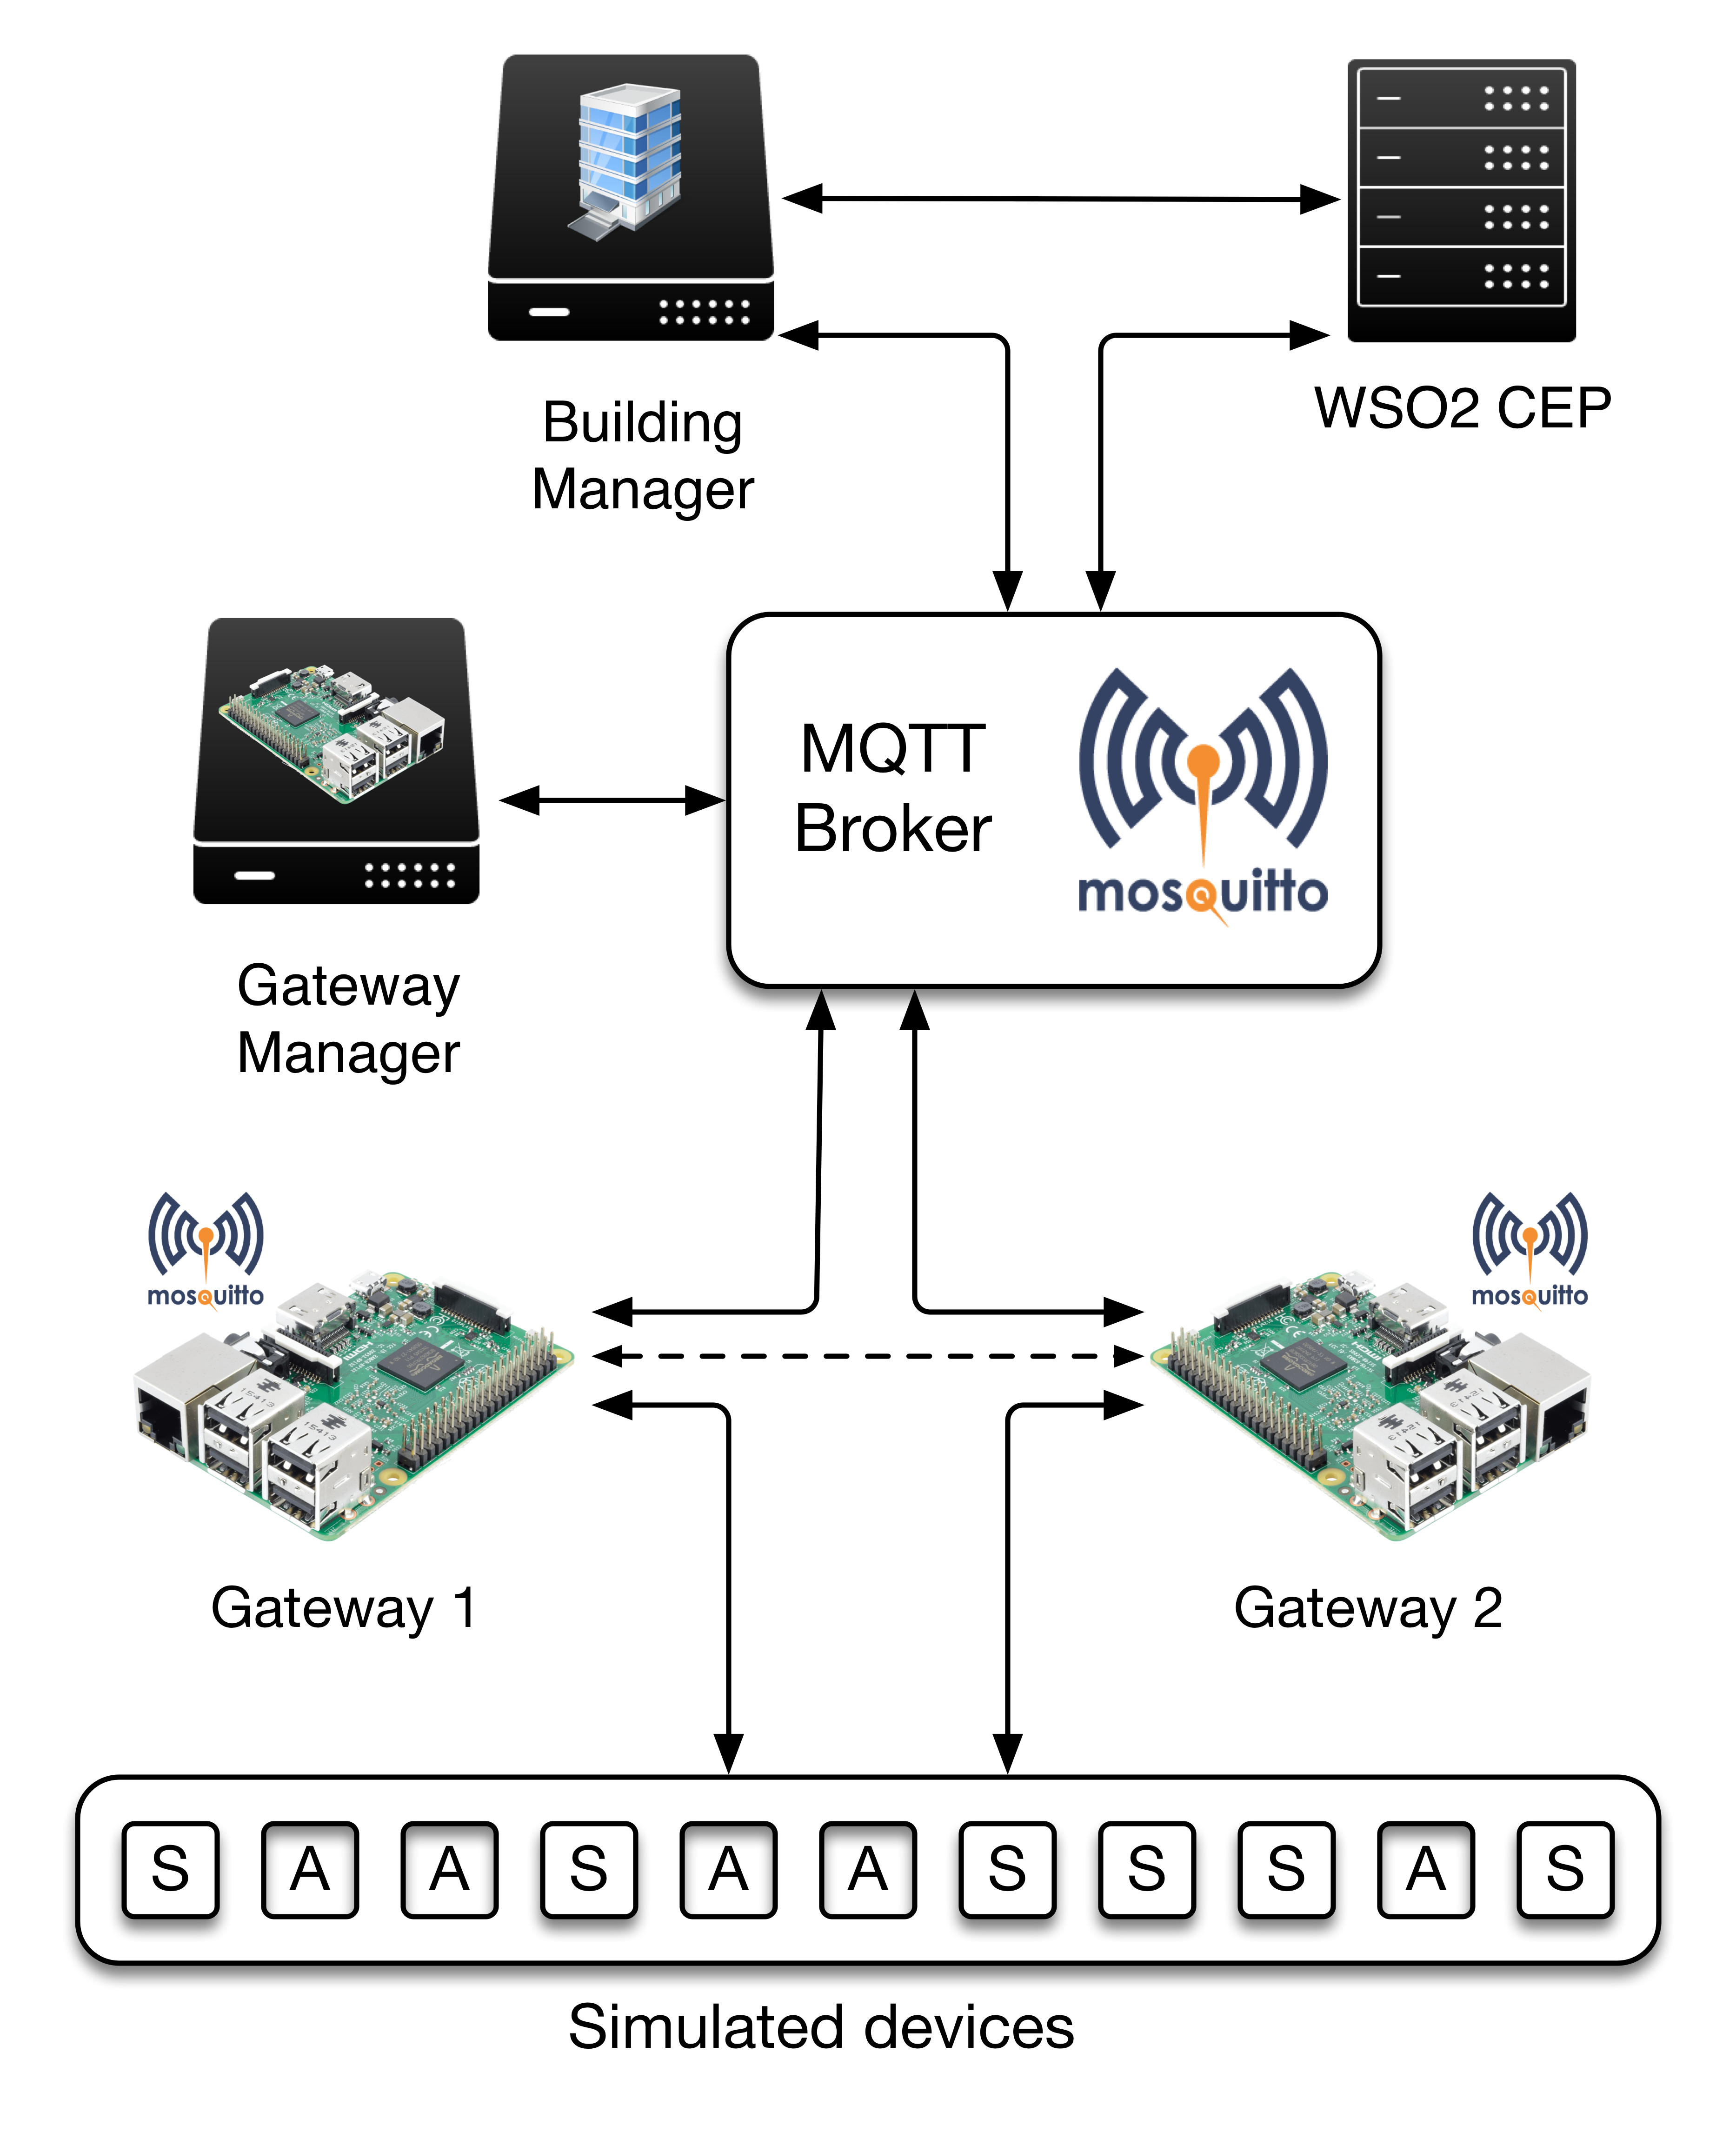
\includegraphics[width=0.7\textwidth]{figures/deployment.png}
	\caption{Deployment Scenario.}
	\label{fig:deploy}
\end{figure}

Regarding the Gateway Manager, it contains both a software for gateway's management and a web-server to offer a platform to check the state of each gateway and the general state of the system. This component was also deployed in a Linux virtual machine with a dual-core processor and 2 gigabytes of memory.

In order to assure the communication between the different components, the Mosquitto MQTT Broker was deployed in a separate virtual machine with a dual-core processor and 2 gigabytes of memory.

Finally, concerning the gateways, which are responsible for communicate with devices and, in some scenarios, process events using its Automation Engine, it was used a Raspberry Pi 3 Model B, which has a quad-core processor with 1 gigabyte of memory \footnote{https://www.raspberrypi.org/products/raspberry-pi-3-model-b/}. 

Regarding the deployment scenario, a equal set of simulated devices were configured in both gateways, simulating a scene where the devices are in range of two different gateways. Each gateway was equipped with code to generate events of the devices assigned to them, by the Gateway Manager. If a gateways had control over a sensor, it should send events with a fixed programmable frequency. This was used for the testing scenario addressed in section \ref{results:fail}. %The simulated devices used were motion sensors and lights actuators and it was deployed a rule, to trigger a light on for 5 seconds, each time a motion sensor sends an event. 

All the tests were done using the internal network of IT Building.




\section{Performance Results}
\label{results:results}

In this section will be presented the results and discussion of the tests preformed. Firstly, in section \ref{results:cep} the latency of the gateway's Automation Engine will be mesured and then, in section \ref{results:fail}, the reaction time to system failures will be evaluated.


\subsection{Gateway's Automation Engine Performance}
\label{results:cep}

In order to evaluate the gateway's Automation Engine performance, a stress test was preformed. The objective was to measure the processing time of events, in five different stress situations: first, sending a single event and measuring the time taken by the engine to produce an output response, and then increasing the number of consecutive events, 10, 100, 1000 and 10000, to not only measure the time taken to process all those events, but also to check if all events were processed. 

For this test, two python scripts were made: one to send a programmable number of events consecutively, and other to measure the time since the first event was sent, and the last response action was received. The deployed rule consisted in inputting a motion event and respond with an event to turn on a light as result. The results of this test are expressed in Figure \ref{fig:performance}.

\begin{figure}[H]
	\centering
	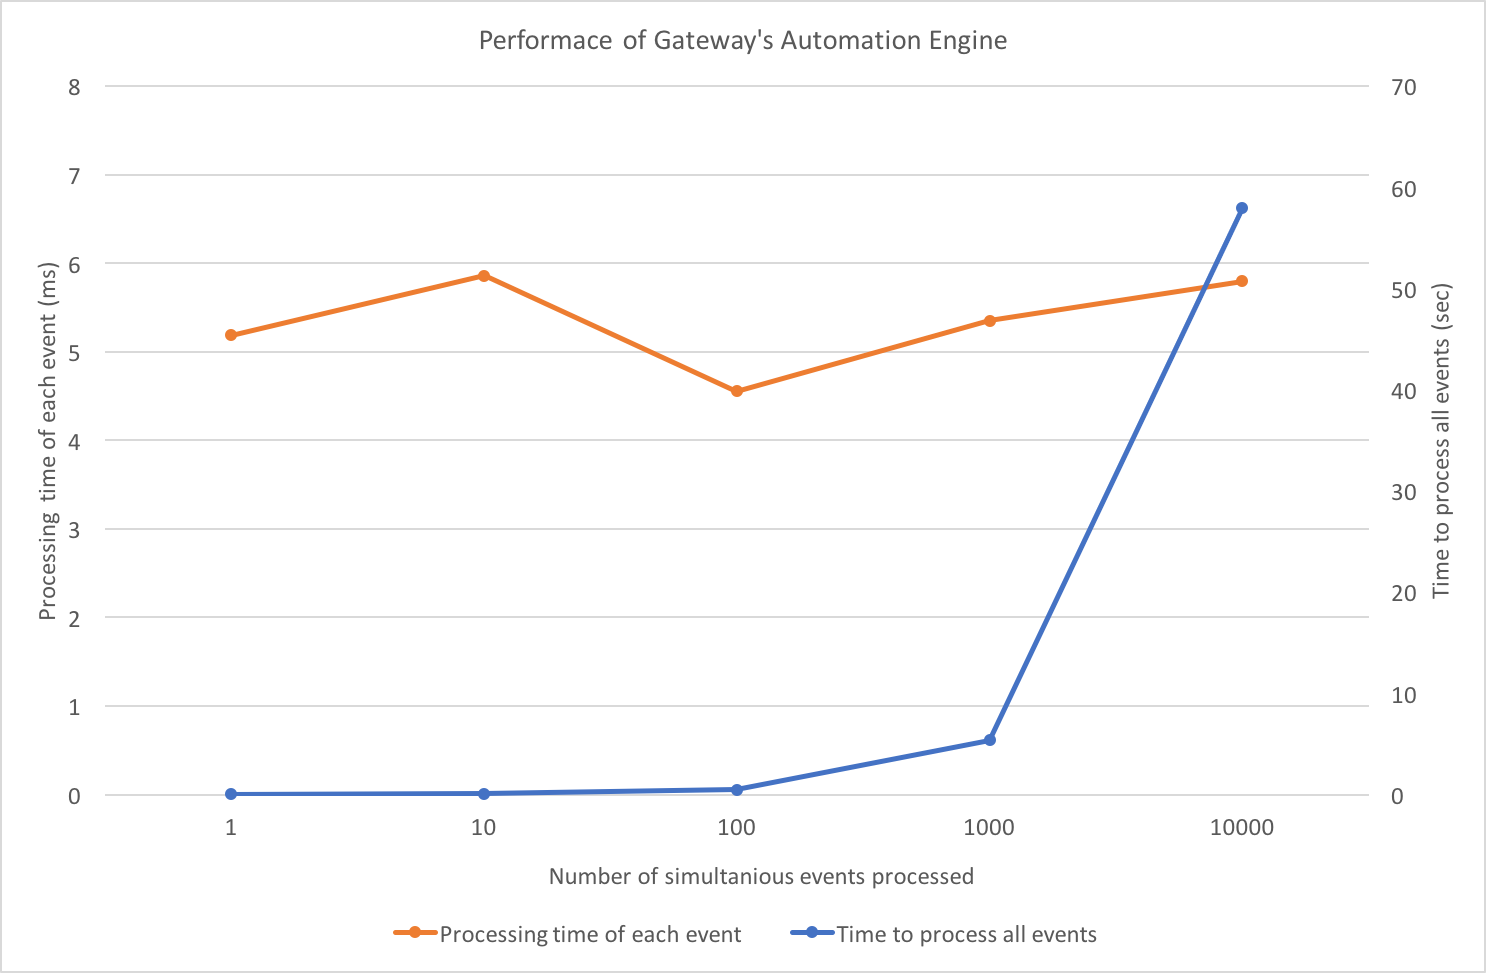
\includegraphics[width=0.9\textwidth]{figures/performance.png}
	\caption{Gateway's Automation Engine Performance.}
	\label{fig:performance}
\end{figure}

As can be observed, the time taken to process each event in the different test scenarios was, in average, between 4 to 6 milliseconds, which is about the same time taken by the WSO2 \ac{cep} Engine, tested in a previous dissertation \cite{helder}, when processing simple rules like the one used for this test. Bellow in table \ref{table:event} are shown more detailed insights about this test.

\begin{table}[H]
	\begin{tabular}{l|l|l|l|l|l|}
		\cline{2-6}
		& \textbf{1} & \textbf{10} & \textbf{100} & \textbf{1000} & \textbf{10000} \\ \hline
		\multicolumn{1}{|l|}{\textbf{Average Time}}       & 5,2 ms     & 5,9 ms      & 4,6 ms       & 5,3 ms        & 5,8 ms         \\ \hline
		\multicolumn{1}{|l|}{\textbf{Minimum Time}}       & 4,4 ms     & 5,6 ms      & 4,5 ms       & 4,5 ms        & 5,5 ms         \\ \hline
		\multicolumn{1}{|l|}{\textbf{Maximum Time}}       & 6,0 ms     & 6,3 ms      & 4,6 ms       & 6,7 ms        & 6,1 ms         \\ \hline
		\multicolumn{1}{|l|}{\textbf{Standard Deviation}} & 0,7 ms     & 0,3 ms      & 0,1 ms         & 0,9 ms        & 0,3 ms         \\ \hline
		\multicolumn{1}{|l|}{\textbf{Total Time}}         & 0,005 sec  & 0,059 sec   & 0,455 sec    & 5,350 sec     & 57,953 sec     \\ \hline
	\end{tabular}
	\centering
\caption{Time taken to process each event.}
\label{table:event}
\end{table}

This test was performed 10 times for each number of simultaneous events. Regarding the time to process each event, it was expected that when increasing the number of simultaneous events, the time needed to process each one of them would increment, since it would increase the processor load, however, as can be observed in Figure \ref{fig:performance}, there is a slight decrease for 100 simultaneous events. This can be explained by the internal architecture of Raspberry Pi's processor and cache.

\subsection{System Failure's Reaction Performance}
\label{results:fail}

In order to test the system reaction to fail scenarios, two tests were done. The first one was to measure the time needed, after a failure in the \ac{cep} engine or in the MQTT Broker, for gateways to enable its automation engine and start processing events. This test addresses the reaction time to scenarios 2,4 and 5, addressed in Chapter \ref{implementation:scenarios}. In these three scenarios, the heartbeat message from the CEP Engine (which that states that this component is running, and thus, there is no need for the gateway's automation engine to be running) stop reaching gateways, either because the CEP Engine actually failed (scenarios 2 and 4), or because the MQTT Broker failed (scenario 5). The scenarios are different, however, the reaction to them is the same for gateways: the gateway's automation engine is enabled and starts processing events. 


 In order to obtain reaction time of gateways to these scenarios, a Python script was made to measure the time since the central \ac{cep} Engine went down (purposely) and the receiving of the first gateway processed result event. Also, input events were being sent to the broker, every 100 milliseconds, this way, after the gateway automation engine was enabled it would receive an input event to process within 100 ms. The obtained results can be consulted bellow, in table \ref{cepDown}.


\begin{table}[H]
	
	\begin{tabular}{|l|l|}
		\hline
		\textbf{Average Time}       & 7,261 sec \\ \hline
		\textbf{Minimum Time}       &  5,084 sec \\ \hline
		\textbf{Maximum Time}       & 8,883 sec \\ \hline
		\textbf{Standard Deviation} & 1,185 sec \\ \hline
	\end{tabular}
	\centering
	\caption{Reaction time to a \ac{cep} Engine failure}
	\label{cepDown}
\end{table}

As can be observer, in average, a gateway needed 5 to 9 seconds to react to the \ac{cep} engine failure. Note that gateways wait for five seconds (configurable timeout) before conclude that the \ac{cep} Engine is down and thus, enable its own automation engine to process events.

Regarding scenario 3, in which there is a failure in the Gateway Manager, no reaction times can be measured, since the failure of this component does not produce any alteration to the normal functioning of the system, i.e. the processing of sensor's generated events.


The second test objective was to measure the time needed to recover from a gateway failure. When a gateway fails, the devices that are in its control become unreachable and thus, the events generated are not published in the broker. The gateway manager, then, needs to check which other gateways have access to those devices and assign them to a new gateway. Also the rules that were deployed in the failing gateway need to be sent to other working gateways. For this test in specific, the same device was configured in two different gateways, and, a event simulator was also implemented in each one of them in order to gateways publish simulated events of the devices they control. To explain further, two gateways were connected with access to the same device, and the Gateway Manager chose one of them to control that device. Then, using a Python script, it was measured the time since the gateway, that was in control of the device, was disconnected, until the other gateway, took over the device and started publishing events. The results of this test were as shown in table \ref{gwdown}

 
\begin{table}[H]

	\begin{tabular}{|l|l|}
		\hline
		\textbf{Average Time}       & 13,194 sec \\ \hline
		\textbf{Minimum Time}       & 7,492 sec \\ \hline
		\textbf{Maximum Time}       & 18,877 sec \\ \hline
		\textbf{Standard Deviation} & 3,839 sec \\ \hline
	\end{tabular}
	\centering
	\caption{Reaction time to a Gateway failure.}
	\label{gwdown}
\end{table}

As can be concluded, by observing the results, the reaction time of a gateway failure is in average 7 to 19 seconds. Note that in this test, gateways were sending heart beats in 5 second intervals, and the the \ac{gm} was checking every 10 seconds whether a gateway was disconnected for more than 10 seconds. That is why there is such a discrepancy between the maximum and minimum values obtained. It depends on when the last heart beat of the failing gateway was sent.

Then, using the same scenario, the disconnected gateway was put back up, and since it was a known gateway for the Gateway Manager, immediately after the first heart beat was received, it attributed the control of the same device back to that gateway. The results, as can be seen in table \ref{gwup}, were from 129 to 199 milliseconds.

\begin{table}[H]
	
	\begin{tabular}{|l|l|}
		\hline
		\textbf{Average Time}       & 0,164 sec \\ \hline
		\textbf{Minimum Time}       & 0,129 sec \\ \hline
		\textbf{Maximum Time}       & 0,199 sec \\ \hline
		\textbf{Standard Deviation} & 0,024 sec \\ \hline
	\end{tabular}
	\centering
	\caption{Reaction time to a Gateway back up.}
	\label{gwup}
\end{table}

\newpage
\begin{Paragraph}{Summary}
	
	
	
To summarize, given these results, the Gateway's Automation Engine is proven to be adequate to be implemented as a back up plan for emergency states where the \ac{cep} Engine might not be reachable. Also since the system is able to react to component's failures within a reasonable time, the requirements and objectives proposed were successfully implemented.  

\end{Paragraph}
